%%
%% licence       kaneton licence
%%
%% project       kaneton
%%
%% file          /home/mycure/kaneton/view/papers/assignments/assignments.tex
%%
%% created       julien quintard   [wed dec  7 16:53:52 2005]
%% updated       julien quintard   [thu jan  5 23:13:20 2006]
%%

%
% template
%

%
% ---------- header -----------------------------------------------------------
%
% project       kaneton
%
% license       kaneton
%
% file          /home/mycure/kaneton/view/template/paper.tex
%
% created       julien quintard   [wed may 16 18:17:37 2007]
% updated       julien quintard   [fri oct  5 07:00:45 2007]
%

%
% class
%

\documentclass[10pt,a4wide]{article}

%
% packages
%

\usepackage[english]{babel}
\usepackage[T1]{fontenc}
\usepackage{a4wide}
\usepackage{fancyheadings}
\usepackage{multicol}
\usepackage{indentfirst}
\usepackage{graphicx}
\usepackage{color}
\usepackage{xcolor}
\usepackage{verbatim}
\usepackage{aeguill}

\pagestyle{fancy}

\setlength{\footrulewidth}{0.3pt}
\setlength{\parindent}{0.3cm}
\setlength{\parskip}{2ex plus 0.5ex minus 0.2ex}

%
% logos
%

\newcommand{\logos}
  {
    \begin{center}
      
\includegraphics[scale=0.8]{\path/logo/kaneton.pdf}
    \end{center}
  }

%
% prototype
%

\newcommand\prototype[2]{
  \begin{tabular}{p{0.2cm}p{13.8cm}}
  & #1
  \end{tabular}

  \begin{tabular}{p{1cm}p{13cm}}
  & #2
  \end{tabular}}

%
% verbatim stuff
%

\definecolor{verbatimcolor}{rgb}{0.00,0.40,0.00}

\makeatletter

\renewcommand{\verbatim@font}
  {\ttfamily\footnotesize\selectfont}

\def\verbatim@processline{
  {\color{verbatimcolor}\the\verbatim@line}\par
}

\makeatother

%
% header
%

\rhead{}
\rfoot{\scriptsize{The kaneton microkernel project}}

\date{\scriptsize{\today}}


%
% header
%

\lhead{\scriptsize{The kaneton microkernel project assignments}}

%
% title
%

\title{The kaneton microkernel project assignments}

%
% authors
%

\author{\small{Julien Quintard}}

%
% prototype
%

\newcommand\prototype[1]{\hspace{1.5cm}#1}

%
% document
%

\begin{document}

%
% title
%

\maketitle

%
% --------- text --------------------------------------------------------------
%

%
% the project
%

\section{The Project}

To get more information about the kaneton project and the kaneton
microkernel reference, please take a look at the kaneton document.

%
% k0
%

\section{k0}

The \textbf{k0} project consists in the development of the bootstrap.

This project is very specific and will not be re-used in the future
projects.

The only goal in the develop a bootstrap in assembly, loading an ELF
binary object from floppy drive into main memory and finally jumping
on the binary entry point.

%
% ia32
%

\subsection{ia32}

The student will have to install and activate the protected mode before
lauching the binary object.

Moreover, the project's diffculty resides in the development of an
application first evolving in real mode, then in protected mode, all
in a single assembly file.

%
% k1
%

\section{k1}

The \textbf{k1} project consists in the development of the bootloader.

This bootloader just relocates the stuff needed by the future kernel
execution.

The relocation is not really necessary but we wanted the students
to understand low-level programming and more especially programming
in a very strict environment with no fine-grain allocator provided.

So in this project, the student has to write the entire code of the
bootloader. The only requirement is to be compliant with the structure
passed to the kernel.

Needless to say, the student will have to install and activate
the protected mode and the virtual memory.

This structure called \textbf{t\_init} is defined in the
file: \textit{core/include/kaneton/init.h}.

The \textit{mem} and \textit{memsz} fields indicate the available physical
memory of the system.

The \textit{kcode} and \textit{kcodesz} fields indicate the location and
size of the kernel binary in main memory.

The \textit{init} and \textit{initsz} fields indicate the location and
size of this init structure in main memory.

The \textit{modules} and \textit{modulessz} fields indicate the
location of the area used to store the modules.

The modules area is composed of:

\begin{enumerate}
  \item
    The number of modules: \textit{nmodules}.
  \item
    An array of modules.
\end{enumerate}

Each module is composed of:

\begin{enumerate}
  \item
    A module structure \textit{t\_module} containing a name and size fields.
  \item
    The module's data: binary, text etc.. depending on the module nature.
  \item
    The module name terminated by a zero character.
\end{enumerate}

The \textit{nsegments}, \textit{segments} and \textit{segmentssz} fields
indicate the area location containing the segment array. This array
describes the core's pre-reserved segments.

The \textit{nregions}, \textit{regions} and \textit{regionssz} fields
indicate the area location containing the region array. This array
describes the segments to be mapped after the initialisation of the
core region manager.

Indeed, many segments will be needless so this array only specify the
fundamental segments to map.

The \textit{kstack} and \textit{kstacksz} fields indicate the kernel
stack area location.

The \textit{alloc} and \textit{allocsz} fields indicate the location
and size of the fine-grain allocator survey area. This area will be
used by the \textit{malloc()} suite functions to provide fine-grain
allocator while no segment neither region manager are initialised yet.

The init structure also contains machine-dependent fields.

The code provided must be located in the directory
\textit{core/bootloader/arch/[architecture]/}.

The students should use the system defines. Be aware that this project
must lead students to understand the project source organisation.

The student will have to build the init structure using the minimum
of memory, the gaming being the pack this structure.

%
% ia32
%

\subsection{ia32}

The physical memory layout for the Intel architecture is the following:

\begin{figure}[h]
\centerline{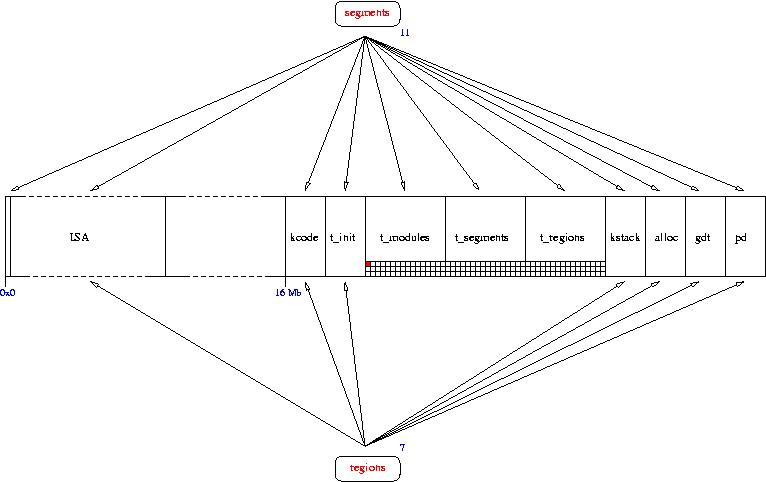
\includegraphics[scale=0.5]{figures/k1-memory-layout.jpg}}
\end{figure}

All the segments must be mapped at the kernel boot time.

Be careful to correctly initialise the machine-dependent fields
including \textit{gdt} and \textit{pd} which will be used by the microkernel
to retrieve the structures in main memory.

%
% k2
%

\section{k2}

The \textbf{k2} project consists in the development of parts of
the microkernel:

\begin{itemize}
  \item
    The id manager.
  \item
    The set manager.
  \item
    The address space manager.
  \item
    The segment manager.
\end{itemize}

%
% id manager
%

\subsubsection{id manager}

The id manager is used to generate identifiers from an identifier object.

Once the identifier object initialised, the identifiers can be generated.

Let's take a look at the id manager functions:

\prototype{t\_error \textbf{id\_show}(o\_id* \textbf{o});}

This function just displays the id object's state.

\prototype{t\_error \textbf{id\_clone}(o\_id* \textbf{o},
                                       t\_id \textbf{old},
                                       t\_id* \textbf{new});}

This function duplicates an id object using the \textbf{o} identifier
object.

\prototype{t\_error \textbf{id\_reserve}(o\_id* \textbf{o},
                                         t\_id* \textbf{i});}

This function reserves an identifier \textbf{i} using the identifier
object \textbf{o}.

\prototype{t\_error \textbf{id\_release}(o\_id* \textbf{o},
                                         t\_id \textbf{i});}

This function releases an identifier.

\prototype{t\_error \textbf{id\_build}(o\_id* \textbf{o});}

This function initialises an identifier object.

\prototype{t\_error \textbf{id\_destroy}(o\_id* \textbf{o});}

This function destroys an identifier object.

\prototype{t\_error \textbf{id\_init}(void);}

This function just initialises the id manager.

\prototype{t\_error \textbf{id\_clean}(void);}

This function just cleans the id manager.

%
% set manager
%

\subsubsection{set manager}

The set manager is used to store data. Every kernel managers use it
instead of building data structures by their own.

The student will have to write the entire code for the \textbf{array} and
\textbf{ll} data structures.

The functions below are explained independently of the data structure.

\prototype{t\_error \textbf{set\_type\_[x]}(t\_setid \textbf{setid});}

This function just returns an error if the set corresponding to
\textbf{setid} is not of the type \textbf{[x]}.

\prototype{t\_error \textbf{set\_show\_[x]}(t\_setid \textbf{setid});}

This function displays a entire set.

\prototype{t\_error \textbf{set\_head\_[x]}(t\_setid \textbf{setid},
                                            t\_iterator* \textbf{iterator});}

This function returns an iterator on the first element of the set.

\prototype{t\_error \textbf{set\_tail\_[x]}(t\_setid \textbf{setid},
                                            t\_iterator* \textbf{iterator});}

This function returns an iterator on the last element of the set.

\prototype{t\_error \textbf{set\_prev\_[x]}(t\_setid \textbf{setid},
                                            t\_iterator \textbf{current},
                                            t\_iterator* \textbf{previous});}

This function returns an iterator on the previous element of the set.

\prototype{t\_error \textbf{set\_next\_[x]}(t\_setid \textbf{setid},
                                            t\_iterator \textbf{current},
                                            t\_iterator* \textbf{previous});}

This function returns an iterator on the next element of the set.

\prototype{t\_error \textbf{set\_insert\_head\_[x]}(t\_setid \textbf{setid},
                                                    void* \textbf{data});}

This function inserts an object at the head of the set.

\prototype{t\_error \textbf{set\_insert\_tail\_[x]}(t\_setid \textbf{setid},
                                                    void* \textbf{data});}

This function inserts an object at the tail of the set.

\prototype{t\_error \textbf{set\_insert\_before\_[x]}(t\_setid \textbf{setid},
                                                      t\_iterator \textbf{iterator},
                                                      void* \textbf{data});}

This function inserts an object before the one specified by the iterator.

\prototype{t\_error \textbf{set\_insert\_after\_[x]}(t\_setid \textbf{setid},
                                                     t\_iterator \textbf{iterator},
                                                     void* \textbf{data});}

This function inserts an object after the one specified by the iterator.

\prototype{t\_error \textbf{set\_add\_[x]}(t\_setid \textbf{setid},
                                           void* \textbf{data});}

This function adds an object in the set.

\prototype{t\_error \textbf{set\_remove\_[x]}(t\_setid \textbf{setid},
                                              t\_id \textbf{id});}

This function removes an object identified by \textbf{id} from the
set \textbf{setid}.

\prototype{t\_error \textbf{set\_delete\_[x]}(t\_setid \textbf{setid},
                                              t\_iterator \textbf{iterator});}

This function deletes the object corresponding to the iterator.

\prototype{t\_error \textbf{set\_flush\_[x]}(t\_setid \textbf{setid});}

This function removes every object stored in the set.

\prototype{t\_error \textbf{set\_locate\_[x]}(t\_setid \textbf{setid},
                                              t\_id \textbf{id},
                                              t\_iterator* \textbf{iterator});}

This function returns an iterator on the element corresponding to the
identifier \textbf{id}.

\prototype{t\_error \textbf{set\_object\_[x]}(t\_setid \textbf{setid},
                                              t\_iterator \textbf{iterator},
                                              void** \textbf{data});}

This function returns the object's data corresponding to the iterator.

\prototype{t\_error \textbf{set\_reserve\_ll}(t\_opts \textbf{opts},
                                              t\_size \textbf{datasz},
                                              t\_setid* \textbf{setid});}

This function reserves a ll set with options \textbf{opts} which will contain
object of \textbf{datasz} size.

\prototype{t\_error \textbf{set\_reserve\_array}(t\_opts \textbf{opts},
                                                 t\_setsz \textbf{initsz},
                                                 t\_size \textbf{datasz},
                                                 t\_setid* \textbf{setid});}

This function reserves an array set with options \textbf{opts}. This
set will contain objects of \textbf{datasz} size and will initialy
be composed of \textbf{initsz} unused elements.

\prototype{t\_error \textbf{set\_release\_[x]}(t\_setid \textbf{setid});}

This function releases a set.

%
% address space manager
%

\subsubsection{address space manager}

The address space manager just manages the address spaces. An address
space is a container describing the addressable memory.

An address space is composed of a set of segments and a set of regions.

\prototype{t\_error \textbf{as\_show}(t\_asid \textbf{asid});}

This function shows a precise address space displaying information
on it.

\prototype{t\_error \textbf{as\_dump}(void);}

This function dumps all the address space managed by the address
space manager.

\prototype{t\_error \textbf{as\_give}(t\_asid \textbf{asid},
                                      t\_tskid \textbf{tskid});}

This function gives an address space to another task.

\prototype{t\_error \textbf{as\_clone}(t\_tskid \textbf{tskid},
                                       t\_asid \textbf{old},
                                       t\_asid* \textbf{new});}

This function clones an address space taking care of cloning everything
necessary.

\prototype{t\_error \textbf{as\_reserve}(t\_tskid \textbf{tskid},
                                         t\_asid* \textbf{asid});}

This function reserves an address space object for the task \textbf{tskid}.

\prototype{t\_error \textbf{as\_release}(t\_asid \textbf{asid});}

This function just releases an address space.

\prototype{t\_error \textbf{as_get}(t\_asid \textbf{asid},
                                    o\_as** \textbf{o});}

This function should only be used by the segment and region managers.

This function just returns the address space object corresponding to
the address space identifier.

\prototype{t\_error \textbf{as\_init}(void);}

This function initialises the address space manager.

\prototype{t\_error \textbf{as\_clean}(void);}

This function cleans the address space manager.

%
% segment manager.
%

The segment manager is used XXX

%
% k3
%

%
% k4
%

%
% k5
%

%
% kn
%



\end{document}
